\documentclass[10pt,twocolumn]{article}
\usepackage[letterpaper,margin=0.72in,columnsep=0.24in]{geometry}
\usepackage[T1]{fontenc}
\usepackage{lmodern,amsmath,amssymb,bm,graphicx,booktabs,microtype}
\usepackage[numbers,sort&compress]{natbib}
\usepackage[colorlinks=true,allcolors=blue]{hyperref}
\usepackage[font=small,labelfont=bf]{caption}
\setlength{\emergencystretch}{1.5em}
\renewcommand{\dbltopfraction}{0.92}
\renewcommand{\textfraction}{0.07}
\renewcommand{\dblfloatpagefraction}{0.65}
\makeatletter
\renewcommand{\maketitle}{\begin{center}\LARGE\@title\end{center}\vspace{0.5em}}
\makeatother
\renewcommand{\thesection}{\Roman{section}}
\renewcommand{\thesubsection}{\Alph{subsection}}
\newcommand{\norm}[1]{\left\lVert#1\right\rVert}
\newcommand{\dd}{\mathrm{d}}
\hypersetup{pdftitle={When Can Hall-Silent Valleys Be Neglected in Anomalous-Velocity Nonlinear Hall Transport?},pdfauthor={}}
\title{When Can Hall-Silent Valleys Be Neglected in\\Anomalous-Velocity Nonlinear Hall Transport?}
\author{}\date{}
\begin{document}
\raggedbottom
\twocolumn[\begin{@twocolumnfalse}\maketitle
\begin{abstract}
A conducting valley with zero direct Berry-curvature Hall weight can still alter the occupation of Hall-active valleys through collisions. We determine when such a sector may be omitted from the anomalous-velocity nonlinear Hall response of a four-valley semiclassical model. Exact sector elimination and a physical hierarchy resolve active reference current, active valley distortion, passive current and passive valley polarization. Contact disorder leaves their four-dimensional space invariant, with three driven amplitudes sufficient in the massless passive limit. Finite-range disorder produces leakage whose observable effect depends on omitted drive, relaxation and signed Hall sensitivity. Four modes reproduce the Hall response within 0.36\% on the tested positive-coupling map. Safe sector omission remains observable and tolerance dependent: at a 1\% Hall tolerance, 40.50\% of safe positive-coupling points depend on favorable cancellation under a fixed-budget test. Finite passive curvature adds direct valley-population readout that can dominate even without intersector coupling. These results explain omission decisions within the specified anomalous-velocity channel, without asserting a complete nonlinear Hall conductivity or a universal material threshold.
\end{abstract}\vspace{0.5em}\end{@twocolumnfalse}]
\section{Introduction}
A time-reversal-invariant conductor can carry a transverse current at second order in an electric field. In the anomalous-velocity contribution, the electric field probes Berry curvature through the first-order nonequilibrium occupation. A constant relaxation time reduces this occupation to velocity times a lifetime, leading to the Berry-curvature-dipole expression~\cite{SodemannFu2015}. The geometric weight and the kinetic distribution then appear almost separable. Microscopic multivalley collisions remove that simplification: carriers can change valley as well as direction, and distinct distortions relax at different rates.

This distinction matters when reducing a multivalley description. Suppose an occupied valley has zero Berry curvature everywhere on its conducting contour. It contributes no direct weight to the anomalous-velocity Hall functional. It nevertheless carries longitudinal current, accepts carriers from other valleys and returns a driven distribution to them. Its absence from the Hall readout does not imply its absence from the kinetic equation. We call such a sector \emph{Hall silent}; the term refers to a specified response channel, not to zero conductivity or to an inert band.

Scattering-induced nonlinear Hall redistribution is already established. Lihm and Park identified valley-polarizing relaxation modes and developed scattering-channel diagnostics, including an exact response difference after channel subtraction~\cite{LihmPark2024}. Multichannel kinetic theories also show why the anomalous-velocity contribution alone need not exhaust the nonlinear Hall response~\cite{NandySodemann2019,Du2019}. We address the narrower question of when an entire conducting, Hall-silent sector may be omitted at a stated tolerance. This differs from asking whether a single relaxation time describes all valleys or whether a particular scattering channel enhances a response.

Our central result is that a zero-curvature conducting valley can remain kinetically indispensable. Safe omission depends on the requested observable, the active and passive relaxation structure, and the accepted error. Within an explicit four-valley model, a contour-weighted projection separates scalar rescaling from Hall-sensitive redistribution. A fixed physical hierarchy and its invariant-subspace residual explain why either contribution can dominate: the relevant competition is between the change in a reference-current amplitude and the excitation of an orthogonal valley distortion with a different Hall overlap and relaxation stiffness. Opposing contributions can also make safe omission cancellation-dependent under a fixed-budget test. We connect that statement to 1\%, 5\% and 10\% decisions, rather than inferring practical significance from a small cancellation factor alone.

The contribution is the use of sector elimination and observable-error analysis in a multivalley omission problem, together with a physically interpretable hierarchy identifying which transport degrees of freedom control the error. The mathematical tools are standard. We use Schur elimination, closely related to Kron reduction of network operators~\cite{DorflerBullo2013}, and an observable-error identity of the adjoint type~\cite{PierceGiles2004}. Their application exposes physical omission mechanisms; no mathematical priority claim is made. A small passive mass supplies a further control: it converts a pre-existing passive valley displacement into direct Hall readout, even without intersector coupling. Finally, ordinary conductivity makes omission of the same sector a different question for an open-circuit signal.

All results concern the anomalous-velocity nonlinear Hall contribution of the specified homogeneous semiclassical model. They do not give a quantitative material prediction, a universal omission threshold, or the complete nonlinear Hall conductivity. The Supplement contains the detailed numerical validation, disorder controls, frequency analysis and sufficient error bounds; the main text develops the physical explanation.

\section{Sector elimination and observable-specific omission}
At zero temperature, let $i$ denote a node on an occupied conduction contour and $w_i>0$ its Fermi-surface integration weight. Write the linearized displacement as $\ell_i$ and use weighted coordinates
\begin{equation}
g_i=\sqrt{w_i}\ell_i,\quad b_i=\sqrt{w_i}v_{x,i},\quad
h_i=\sqrt{w_i}\Omega_{z,i}.
\end{equation}
For elastic, reversible Born rates $\mathcal W_{ij}=\mathcal W_{ji}\geq0$, the symmetrized collision operator is
\begin{equation}
L_{ij}=\delta_{ij}\sum_k\mathcal W_{ik}w_k
-\sqrt{w_iw_j}\mathcal W_{ij}.\label{eq:L}
\end{equation}
It is positive semidefinite and conserves charge. The drive and Hall weight are odd under time reversal, so their response can be solved in the invariant odd subspace, excluding the even conserved charge modes without adding a relaxation rate. In this space
\begin{equation}
(L+i\omega I)g=b,\qquad H=h^Tg.\label{eq:response}
\end{equation}
With $E_x(t)=\operatorname{Re}(E_0e^{i\omega t})$, the second-harmonic coefficient in units $e=\hbar=1$ is $\chi_{yxx}=-H/2$. DC results below mean its $\omega\to0$ limit. The transpose in Eq.~\eqref{eq:response} is bilinear, not a complex-conjugate inner product.

Partition the projected operator and drive into Hall-active ($A$) and passive ($P$) sectors:
\begin{equation}
\begin{pmatrix}A&B\\B^T&F\end{pmatrix}
\begin{pmatrix}g_A\\g_P\end{pmatrix}
=\begin{pmatrix}b_A\\b_P\end{pmatrix},\qquad h_P=0.
\end{equation}
The condition $h_P=0$ imposes neither $b_P=0$ nor $B=0$: a Hall-silent sector can be driven and collision coupled. Here $A,F$ include $i\omega I$ when needed. Eliminating the passive displacement gives
\begin{align}
\Sigma_P&=BF^{-1}B^T,&\zeta_P&=BF^{-1}b_P,\\
M&=A-\Sigma_P,&g_A&=M^{-1}(b_A-\zeta_P).\label{eq:schur}
\end{align}
The sector changes both the active relaxation operator and its effective drive. Retaining only its scattering-out rate would miss the second effect and the return term $\Sigma_P$.

The omission reference removes every active--passive scattering edge, including its diagonal loss. Let $A_{\rm ref}$ be the resulting active operator and
\begin{equation}
g_{A0}=A_{\rm ref}^{-1}b_A,\qquad H_0=h_A^Tg_{A0}.
\end{equation}
This is a microscopic active-only problem, not a lifetime fit. With $\Delta_A=A-A_{\rm ref}$, subtraction yields
\begin{align}
f&=(\Delta_A-\Sigma_P)g_{A0}+\zeta_P,\\
g_A-g_{A0}&=-M^{-1}f,\\
\Delta H&=H-H_0=-h_A^TM^{-1}f.\label{eq:exacterror}
\end{align}
Equation~\eqref{eq:exacterror} shows explicitly why $h_P=0$ does not imply $\Delta H=0$. Passive kinetics is sampled indirectly through the changed active distribution. Conversely, a large displacement change need not cause a large Hall error if it has little overlap with $h_A$.

We define the relative omission using the full response:
\begin{equation}
e_H=\frac{|H-H_0|}{|H|}.\label{eq:error}
\end{equation}
A sector is safe to omit at tolerance $\epsilon$ when $e_H\leq\epsilon$, provided the denominator is well conditioned. An error exceeding unity is possible if the retained response is much larger than the full one. Ratios with nearly vanishing $H$ or $H_0$ must instead be described by absolute errors; no such ambiguous principal-map points occur here.

For completeness, $M^Tz=h_A$ gives the exact signed identity $\Delta H=-z^Tf$ and sufficient bounds
\begin{equation}
|\Delta H|\leq\norm z\norm f
\leq\frac{\norm{h_A}\norm f}{s_{\min}(M)}.
\end{equation}
Any absolute bound $E<|H_0|$ implies $e_H\leq E/(|H_0|-E)$. Once the exact $z$ and $f$ are available, however, their contraction already gives the correction. These inequalities support conservative decisions; they are not the central physical result or a demonstrated dense-solver acceleration. Their coverage and cost are assessed in the Supplement.

\section{Physical four-mode transport theory}
\subsection{Symmetry and the fixed mode hierarchy}
The hierarchy first retains the active current response, then an independent active valley displacement, then passive current and finally passive valley polarization. These coordinates distinguish carrying current from changing the partner populations. We construct a physical real basis from the DC reference and hold it fixed in frequency. Let $p_r=\sqrt w\,s\,1_r$ denote the weighted partner-population displacement in sector $r$, implicitly projected into the orthonormal time-reversal-odd coordinates. Starting from
\begin{gather}
U_{\rm raw}=(g_{A0},p_A,b_P,p_P),\nonumber\\
U=U_{\rm raw}\mathsf T,\quad U^TU=I.\label{eq:basis}
\end{gather}
we orthonormalize in this order. Sector-supported vectors are embedded with zeros in the other sector. Thus $u_1=g_{A0}/G$, $G=\norm{g_{A0}}$, and $u_2$ is the normalized component of $p_A$ orthogonal to $u_1$. The passive columns are normalized current and partner population. Their overlap vanishes for the untilted passive contour used here. The saved matrix $\mathsf T$ specifies every normalization and subtraction.

The first column is the full uncoupled current response, not generally $v_x$ times a lifetime. It retains the active sector's own non-scalar relaxation. The second column therefore describes an independent active valley distortion; after orthogonalization it need not be a pure population or have zero current overlap. The passive current has zero partner-population difference, while the fourth column changes the populations with opposite signs. Neither is a total active-to-passive charge-transfer mode, which is even under time reversal and absent from the driven space.

For the Hamiltonian of Sec.~IV, time reversal sends $(s,q_x,q_y)$ to $(-s,-q_x,-q_y)$. The remaining physical mirror sends it to $(-s,-q_x,q_y)$ with internal action $\sigma_x$. All four displacements are odd under both operations and even under their combined local $q_y$ reflection. Simple partner exchange at equal local angle is not a symmetry of the tilted active contours; assigning its parity to the active columns would be incorrect. Figure~\ref{fig:model} summarizes the physical content.

Models M1--M4 retain the first one through four columns, without changing their order or fitting additional harmonics. For $U_m=(u_1,\ldots,u_m)$,
\begin{align}
K_m&=U_m^TLU_m,\quad d_m=U_m^Tb,\quad j_m=U_m^Th,\nonumber\\
(K_m+i\omega I)x_m&=d_m,\quad g_m=U_mx_m,\quad H_m=j_m^Tx_m.
\end{align}
Every projection uses the same full collision operator. In particular, M1 and M2 retain intersector scattering-out even though passive displacement is frozen; they are not the active-only omission reference. Incremental differences $H_m-H_{m-1}$ describe this ordered ablation, not independent scattering-channel contributions.

We also evaluate $\sigma_{xx,m}=b^Tg_m$, $\chi_m=-H_m/2$ and
\begin{equation}
Q=\frac{H W}{\sigma_{xx}D},\qquad
Q_A=\frac{H W_A}{\sigma_A D},\label{eq:Q}
\end{equation}
where $D=h^Tb$, $W=b^Tb$, $W_A=b_A^Tb_A$ and $\sigma_A=b_A^Tg_A$. These ratios compare Hall readout with current relaxation. Projection errors use the full observable as denominator, distinct from the omission error in Eq.~\eqref{eq:error}. Distribution error is $\norm{g_m-g}/\norm g$ in weighted coordinates. The $x$-driven basis is not used to approximate the different symmetry sector driven by $v_y$.

\begin{figure*}[!tp]\centering
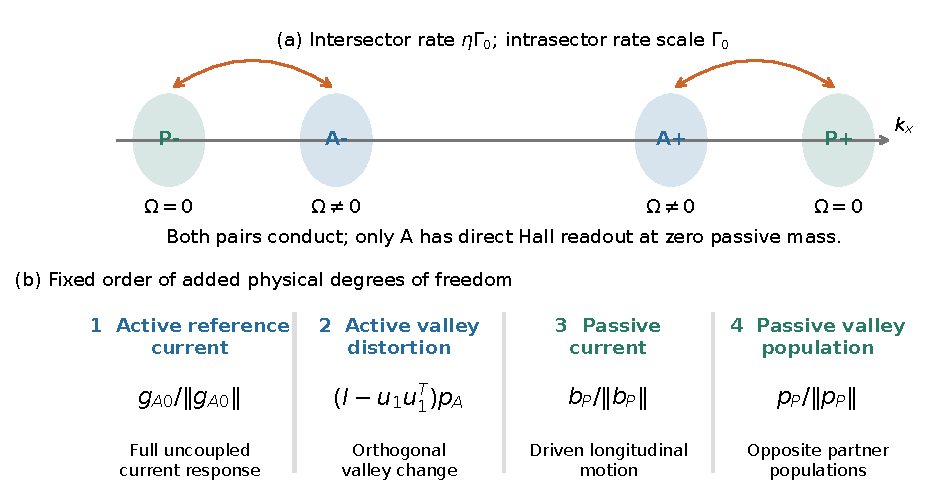
\includegraphics[width=\textwidth]{../figures/main/figure_1_physical_modes.pdf}
\caption{Model and physical coordinates. (a) Hall-active and Hall-silent conducting pairs with intra- and intersector scattering; the contours are schematic. (b) The fixed sequence of physical degrees of freedom. The active distortion is normalized after removing its reference-current component. The passive modes have zero direct Hall weight at $m_P=0$, but can transmit drive and relaxation changes to the active pair. All columns use the contour-weighted inner product.}\label{fig:model}
\end{figure*}

\subsection{Contact closure and finite-range leakage}
For contact disorder, $|u_i^\dagger u_j|^2=(1+\bm n_i\cdot\bm n_j)/2$. Time reversal cancels each sector's integrated Bloch vector, so scattering out has the constant rate $\Gamma_0(D_r+\eta D_{\bar r})/2$, where $D_r$ is its density of states. The constant incoming moment vanishes for an odd displacement. On a contour $\delta=\mu-E=stq_x+d$,
\begin{align}
n_y&=(v_x-st)/v,\\
n_z&=\frac m\delta\left[s(1-t^2/v^2)+(t/v^2)v_x\right].\label{eq:closure}
\end{align}
The remaining component $n_x=-vq_y/d$ is odd under local $q_y$ reflection and does not enter this drive sector. Incoming moments therefore close on the two functions $v_x,s$ in each sector. This space contains the drive and is invariant under $L$. Replacing active velocity by its uncoupled response leaves the same span. At $m_P=t_P=0$, the passive population has zero drive and decouples, so M3 already solves the contact problem exactly. Finite range makes the outgoing rate angle dependent and prevents the incoming kernel from factoring into this finite set of moments.

With $P_U=UU^T$, define
\begin{align}
R_{\rm inv}&=(I-P_U)LU,\\
\rho_{\rm abs}&=\norm{R_{\rm inv}}_2,&
\rho_{\rm rel}&=\frac{\norm{R_{\rm inv}}_2}{\norm{LU}_2}.\label{eq:leak}
\end{align}
Both are spectral norms; separate Frobenius diagnostics are supplied. Closure is a property of the operator and basis, not a synonym for an accurate observable.

The drive can also miss the finite-range space. For $b_\perp=(I-P_U)b$, the reduced residual and exact response error obey
\begin{align}
r_b&=b-(L+i\omega I)Ux_4=b_\perp-R_{\rm inv}x_4,\\
H-H_4&=h^T(L+i\omega I)^{-1}r_b=z^Tr_b.\label{eq:projectionerror}
\end{align}
Here $(L+i\omega I)^Tz=h$ and $U^Tr_b=0$. Consequently $z$ may be replaced by $(I-P_U)z$. At DC a rigorous estimate is
\begin{equation}
|H-H_4|\leq\norm{(I-P_U)z}\norm{r_b}
\leq\frac{\norm{r_h}\norm{r_b}}{\lambda_{\min}(L)},\label{eq:dualbound}
\end{equation}
where $r_h=h-LU K_4^{-1}U^Th$ is the Galerkin dual residual; the second inequality follows by subtracting the reduced dual solution before projection. In turn $\norm{r_b}\leq\norm{b_\perp}+\rho_{\rm abs}\norm{x_4}$. Thus leakage alone cannot bound Hall error without drive, relaxation and readout information. These standard residual estimates explain the diagnostics; no computational advantage is inferred from an exact dual solve.

\subsection{Scalar and Hall-sensitive redistribution}
At DC the active reference defines the exact decomposition
\begin{align}
\alpha_*&=\frac{g_{A0}^\dagger g_A}{g_{A0}^\dagger g_{A0}},\qquad r_A=g_A-\alpha_*g_{A0},\nonumber\\
H-H_0&=S+T,\quad S=(\alpha_*-1)H_0,\quad T=h_A^Tr_A.\label{eq:ST}
\end{align}
The terms $S$ and $T$ are projection-defined diagnostic components, not independently measurable microscopic currents. Their separation depends on the stated contour norm and active reference. In M4, $S_4=j_1(x_1-G)$ and $T_4=j_2x_2$: the active valley distortion is the retained shape coordinate. Eliminating the two passive coordinates gives
\begin{equation}
\begin{pmatrix}a&c\\c&d\end{pmatrix}\binom{x_1}{x_2}
=\binom{p_1}{p_2}.\label{eq:shapeamp}
\end{equation}
Then $x_2=(p_2-cp_1/a)/\kappa$ with $\kappa=d-c^2/a$. Passive feedback changes the effective rates, and transmitted passive drive changes both entries of $p$. The shape response is a residual forcing divided by a positive Schur stiffness and multiplied by its Hall overlap. The stiffness is not itself a collision eigenvalue. This representation predicts scalar or shape dominance from amplitudes and readout, while allowing their signed contributions to oppose.

\section{Four-valley model and collision dynamics}
\subsection{Bands and Hall readout}
Each sector has time-reversed partners $s=\pm1$, centered at $\bm K_{A,s}=(6s,0)$ and $\bm K_{P,s}=(12s,0)$. Local momentum is $\bm q=\bm k-\bm K_{r,s}$. We use
\begin{equation}
\mathcal H_{r,s}(\bm q)=(E_r+st_rq_x)I
-v_rq_y\sigma_x+v_rq_x\sigma_y+sm_r\sigma_z.
\end{equation}
The upper-band energy and Berry curvature are
\begin{align}
\varepsilon_{r,s}&=E_r+st_rq_x+d_r,\quad
 d_r=\sqrt{m_r^2+v_r^2q^2},\\
\Omega_{r,s}&=-\frac{s m_rv_r^2}{2d_r^3}.
\end{align}
The curvature convention is $\bm{\mathcal A}=i\langle u|\nabla_{\bm q}u\rangle$. We set $\mu=1.8$, $E_A=0$, $m_A=1$, $t_A=0.15$, $v_A=v_P=1$, and $t_P=0$. The passive occupation is $\delta_P=\mu-E_P$. Unless stated otherwise, $m_P=0$, so the passive contour conducts but has identically zero curvature. The symmetries permit a passive mass; Hall silence is an imposed band limit, not symmetry protection.

The active and passive local cutoffs are $q<2.5$. Throughout the sampled domain $\delta_P=0.4$--$1.2$, the contours enclose their origins, stay separated and lie within the cutoffs. The active tilt allows a Hall response to an $x$-directed field. Both partners are retained: their equilibrium Hall integrals cancel, whereas their driven contributions can add. Figure~\ref{fig:model} distinguishes this readout from the collision architecture.



\subsection{Disorder and the kinetic distinction}
The collision rates are
\begin{equation}
\mathcal W_{ij}=\Gamma_0 a_{r_ir_j}
 F_\xi(|\bm k_i-\bm k_j|^2)|u_i^\dagger u_j|^2,
\label{eq:rates}
\end{equation}
where $a_{AA}=a_{PP}=1$, $a_{AP}=a_{PA}=\eta$, and $\Gamma_0=0.01$. Thus $\eta$ scales an intersector \emph{rate}, not a signed amplitude. The principal map uses $F_\xi(Q^2)=\exp(-\xi^2Q^2)$ with $\xi=0,0.05,0.10$. The mode-ablation comparison also uses $F_\xi(Q^2)=(1+\xi^2Q^2)^{-1}$. At $\xi=0$ the two kernels are identical.

These rates follow from independent real Gaussian fields coupled to the two diagonal sector projectors and to an intersector hybridization matrix, all scalar in the common two-component internal basis. Their spectral covariances are proportional to $1,1,\eta$, respectively, times $F_\xi$. Valley projection supplies the full momentum transfer in Eq.~\eqref{eq:rates}; the Born energy delta function is absorbed in $w_i$. The Supplement gives the explicit construction and its assumptions. Positive radial kernels make the covariance realizable, but do not identify a particular material's defect ensemble.

There are two distinct ways for this disorder to affect a Hall response. It can change how much of a current-like active distribution survives, and it can redistribute the occupation toward a different Hall-sensitive active pattern. Both processes can be present in the active-only problem. The question here is the additional change produced by coupling to the passive sector, with the same active bands and intrasector disorder held fixed.

The principal map contains 3600 points, of which 3510 have positive coupling: 30 passive occupations, three ranges and 40 couplings including zero. Positive $\eta$ spans $10^{-3}$--10; each contour has $N=256$ nodes. Validation and convergence of the underlying transport solver are summarized in the Supplement. The rate envelope remains below 0.05 of the minimum interband gap. This establishes a scale hierarchy within the model, not a five-percent error bound or a justification for dropping other Hall channels.

The additional kernel comparison uses five occupations $0.4,0.6,0.8,1.0,1.2$, three ranges and ten couplings for each kernel. Identical contact cases are counted once in summaries, giving 250 distinct points, including 225 at positive coupling. This fixed comparison tests the physical hierarchy without adjusting its columns.

\section{Results}
\subsection{What each added mode changes}
Figure~\ref{fig:ablation} compares the hierarchy at four fixed points: weak finite-range coupling $(\eta,\delta_P,\xi)=(0.001,0.4,0.1)$; strong contact coupling $(10,1.2,0)$; a shape-dominated contact case $(0.372759\ldots,0.4,0)$; and a finite-range fixed-budget cancellation case $(0.263665\ldots,0.510345\ldots,0.1)$. Their mechanism labels concern the full solution, not a criterion for choosing the basis.

The first two columns expose why Hall sensitivity and ordinary conduction must be separated. M1 has no orthogonal active shape coordinate. Adding $u_2$ changes the active Hall readout strongly in the scalar example, reducing Hall error from 31.92\% to 0.681\%. Nevertheless its conductivity error remains 62.98\%, because passive current is frozen. In the contact shape example, M2 instead worsens Hall error from 2.063\% to 3.056\%. A physically meaningful added degree of freedom need not improve every functional monotonically. The variational property of a positive collision operator controls its energy norm, not the signed Hall functional.

M3 restores passive current. Both contact examples then agree with the full distribution within numerical precision, as the closure argument predicts. Thus passive current can transmit a Hall correction while having no Hall weight itself; its role is not confined to conductivity. The fourth mode contributes zero in this contact, massless limit.

Finite range changes the result. At the cancellation point, M1, M2 and M3 have Hall errors 4.146\%, 8.855\% and 16.869\%, respectively. M3 has already reduced conductivity error to 0.477\%. Adding passive valley polarization changes $H$ by $-0.966206$ and reduces Hall error to 0.01062\%; $Q_A$ error is 0.01152\%, while distribution error remains 1.894\%. The passive population thus supplies a distinct feedback pathway that ordinary conduction alone does not resolve. At the matched finite-range point $(1,1.2,0.05)$, M3 and M4 Hall errors are 7.095\% and 0.01207\%, confirming that the need for this mode is not confined to the near-cancellation example.

Conversely, at the weak point M1 already predicts $H$ to 0.0153\%, but misses conductivity by 74.56\% and the full distribution by 98.20\%. Four modes are not required there for a one-percent Hall prediction. They are required within this hierarchy for a common accurate description of the harder finite-range cases and of more than one observable. This conclusion concerns the tested ordered models, not a proof against every possible three-dimensional basis.

\begin{figure*}[!tp]\centering
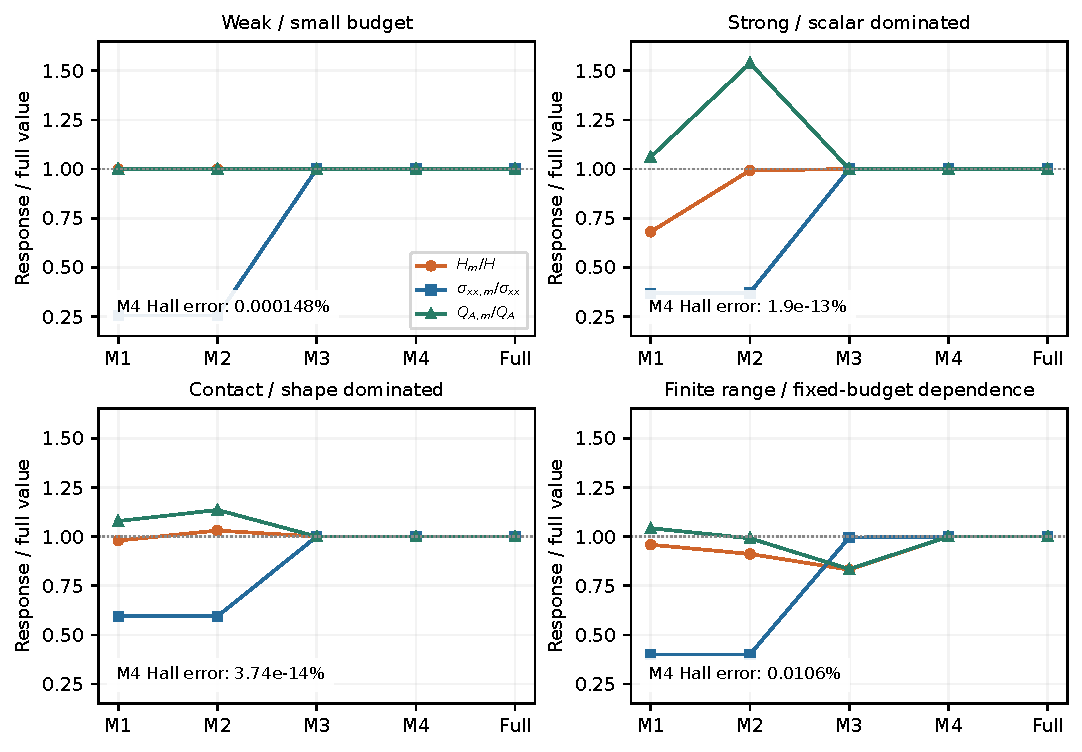
\includegraphics[width=\textwidth]{../figures/main/figure_2_ablation.pdf}
\caption{Physical mode ablation. Each panel compares normalized $H$, $\sigma_{xx}$ and $Q_A$ for M1--M4 and the full solution at the four points specified in Sec.~V.A. M1 is active reference current; M2 adds active valley distortion; M3 adds passive current; M4 adds passive valley population. All project the same full operator. Nonmonotonic Hall convergence is physical and is retained. Contact M3 is exact within numerical precision; finite-range M4 is approximate. Gaussian kernel, $m_P=0$, $N=256$ and common internal texture throughout.}\label{fig:ablation}
\end{figure*}

Across all 3510 positive-coupling principal-map points, M4's 95th-percentile and maximum relative Hall errors are 0.07267\% and 0.35751\%. Its maximum $\sigma_{xx}$ and $Q_A$ errors are 0.39543\% and 0.14630\%; its maximum weighted distribution error is larger, 4.58492\%. All 3510/3510 points meet one-percent accuracy for these three observables, whereas M3 meets that Hall criterion at only 1950/3510 points (55.56\%). Projection accuracy and sector-omission safety remain different questions: using M4 to estimate omission reproduces 3510/3510 decisions (100\%) at both 1\% and 5\%, and 3509/3510 (99.97\%) at 10\%. The one disagreement is false unsafe. These are sampled agreements, not certificates at unsampled boundaries.

\subsection{Closure, leakage and observable error}
Contact closure is analytic and numerical: the largest principal-map $\rho_{\rm rel}$ is $7.40\times10^{-15}$. On the positive-coupling two-kernel comparison, Gaussian finite-range residuals span $0.00648$--$0.03148$ at $\xi=0.05$ and $0.01512$--$0.06798$ at $\xi=0.10$. The corresponding Lorentzian intervals are $0.00536$--$0.02286$ and $0.01099$--$0.04736$. These are nonzero departures from an invariant space, not exact finite-range closure. Figure~\ref{fig:leakage} relates them to the projected response.

Leakage is informative but incomplete. Across the 2340 positive-coupling Gaussian finite-range points, its Spearman correlations with Hall, distribution and $Q_A$ errors are 0.606, 0.555 and 0.573. For Hall error the correlation changes from 0.774 at $\xi=0.05$ to 0.389 at $\xi=0.10$. Increasing leakage thus accompanies degradation in aggregate, but does not define a single error law. Equation~\eqref{eq:projectionerror} explains why: the omitted drive can compensate leakage forcing, and their residual must be weighted by the inverse collision operator and Hall readout.

The weak example makes the first effect explicit. The norms of $b_\perp$ and $R_{\rm inv}x_4$ are 0.00930086 and 0.00931814, but their difference has norm $8.07\times10^{-5}$. Most Frobenius leakage power lies above the median collision rate, and those leaked high-rate modes have small Hall overlap. Their combined response error is $-8.56\times10^{-6}$. This mechanism is consistent with the basis containing the exact uncoupled active response, despite a nonzero projection miss of the drive.

The difficult finite-range cases do not share a universal fast-mode explanation. At the matched Gaussian and Lorentzian points only 9.12\% and 8.18\% of leakage power lies above the median rate. At the cancellation point the exact spectral expansion
\begin{equation}
H-H_4=\sum_\nu\frac{(h^Tv_\nu)(v_\nu^Tr_b)}{\lambda_\nu}
\label{eq:spectralerror}
\end{equation}
has sum of absolute terms 0.301629 but signed sum $-0.000608821$. The full eigenmodes $v_\nu$ need not individually lie outside $U$; the leakage vector does. Degenerate subspaces are interpreted through summed residues. The Supplement displays leakage, drive and Hall weights.

Galerkin orthogonality gives another useful description. The exact Hall dual lies close to the retained space: $\norm{(I-P_U)z}/\norm z=0.00346$ at the cancellation point. Its orthogonal-residual bound in Eq.~\eqref{eq:dualbound} is 0.00394, compared with actual absolute error 0.000609. The simpler primal--dual residual bound is 0.0366 and is conservative. Accuracy therefore reflects a small omitted output sensitivity and signed modal compensation, not merely a small operator norm or uniformly fast leaked modes. These diagnostics do not establish robustness under arbitrary changes of bands or disorder.

\begin{figure*}[!tp]\centering
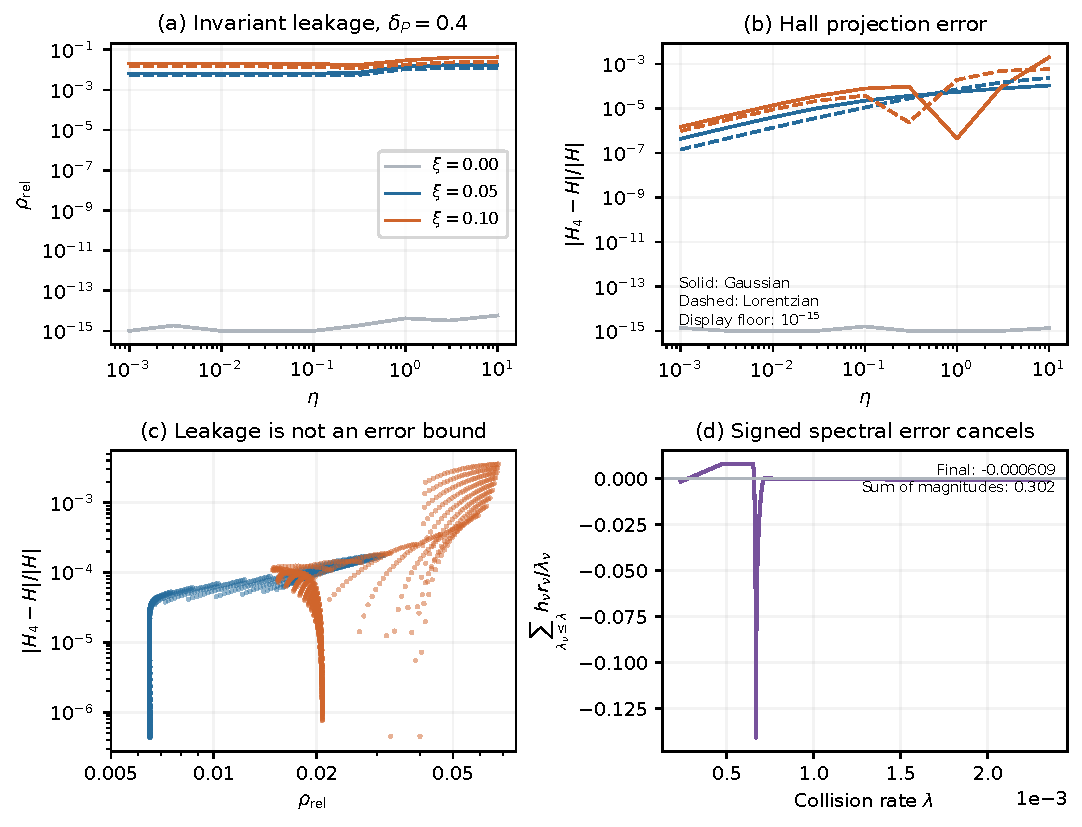
\includegraphics[width=\textwidth]{../figures/main/figure_3_leakage.pdf}
\caption{Invariant leakage and response accuracy. (a,b) Spectral residual and relative Hall error at $\delta_P=0.4$ on the fixed two-kernel grid; values below $10^{-15}$ are displayed at that floor. (c) All 2340 positive-coupling finite-range principal-map points. Each range contains 1170 points. Leakage is correlated with error but is not a bound. (d) Cumulative signed contributions to Eq.~\eqref{eq:spectralerror} at the fixed-budget cancellation point. The small final error results from compensated mode residues. All calculations use the fixed four-column basis and $N=256$.}\label{fig:leakage}
\end{figure*}

\subsection{Scalar, shape and signed compensation}
Define the component budget and cancellation diagnostics
\begin{align}
a&=|S|+|T|,\qquad B=a/|H_0|,\nonumber\\
f_{\rm sh}&=|T|/a,\qquad C=|S+T|/a.
\end{align}
Fractions are undefined at zero budget. We describe a nonzero correction as scalar or shape dominated when that component supplies at least 80\% of the absolute budget. These descriptive labels do not decide whether omission is safe.

For strong contact coupling, $S=2.23807$ and $T=0.0219153$: 99.03\% is scalar. The shape representative has $S=0.0472734$ and $T=0.190306$, or 80.10\% shape. The contact Hall overlaps are the same, $j_1=-0.0112813$, $j_2=-0.0643947$, so the active valley distortion has 5.708 times the readout per unit norm. The scalar case changes the reference amplitude by $-198.387$, with distortion amplitude $-0.340328$. In the shape case these are $-4.19040$ and $-2.95531$. Their residual shape forcings are comparable, but the shape case's stiffness is $0.00227649$, versus $0.0210367$ for the scalar case. A more weakly relaxed, Hall-sensitive distortion can therefore dominate a much smaller scalar change. The passive modes transmit the drive and feedback that set this competition.

At the finite-range cancellation point the reference-current amplitude increases while the active distortion has the opposite sign. Negative Hall overlaps then produce $S=-0.186970$ and $T=0.241183$. Figure~\ref{fig:mechanisms} compares these mechanisms with the weak, small-budget case. Cancellation between $S,T$ concerns the omission correction; cancellation among Eq.~\eqref{eq:spectralerror}'s residues concerns the projection error. They are distinct decompositions and should not be conflated.

\begin{figure*}[!tp]\centering
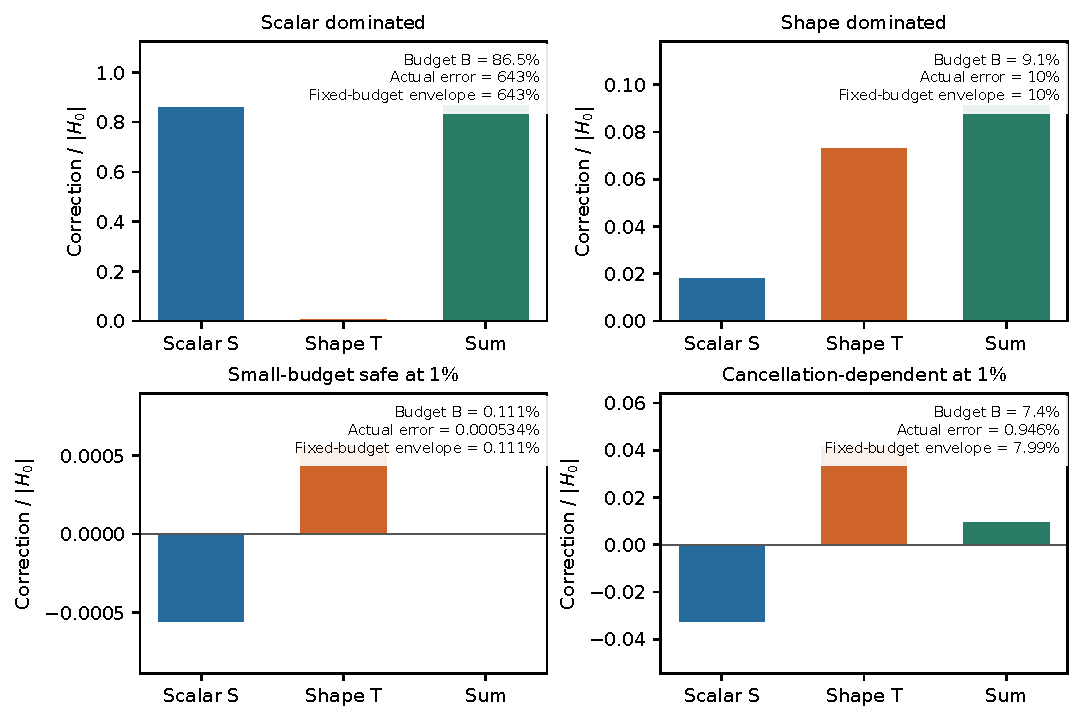
\includegraphics[width=\textwidth]{../figures/main/figure_4_scalar_shape.pdf}
\caption{Scalar and redistribution contributions to omission at the same four representative points as Fig.~\ref{fig:ablation}. Bars retain the signs of $S,T$ and their sum; annotations give the absolute budget, actual omission error and fixed-budget envelope. Strong cancellation at the weak point is irrelevant to a 1\% tolerance because its entire budget is small. The finite-range example is instead cancellation-dependent under the fixed-budget test at 1\%. Vertical scales differ to resolve each signed budget.}\label{fig:mechanisms}
\end{figure*}

\subsection{Tolerance decisions under the fixed-budget test}
Keep $|S|$ and $|T|$ fixed and ask whether removing their favorable signed cancellation could exceed the tolerance. For a possible net correction $D_c$ in $|D_c|\leq a$, the sharp interval/disk envelope is
\begin{equation}
e_{\rm fb}=\sup\frac{|D_c|}{|H_0+D_c|}
=\begin{cases}B/(1-B),&B<1,\\\infty,&B\geq1.\end{cases}\label{eq:envelope}
\end{equation}
For two real fixed magnitudes the discrete sign set is $\{\pm a,\pm(|S|-|T|)\}$. Its maximum agrees with this envelope for $B<1$, but need not diverge for $B\geq1$; both are saved. The test does not imply robustness to arbitrary physical perturbations, which can change the magnitudes themselves.

A well-conditioned point is robustly safe when $e_H\leq\epsilon$ and $e_{\rm fb}\leq\epsilon$. It is \emph{cancellation-dependent under the fixed-budget test} when $e_H\leq\epsilon<e_{\rm fb}$, and unsafe when $e_H>\epsilon$. Every dependent point here has opposing signs and $B<1$, so the discrete-sign and interval decisions coincide. Table~\ref{tab:decisions} reports the principal statistics using only $\eta>0$; zero-coupling controls are excluded.

\begin{table*}[t]\centering\small\setlength{\tabcolsep}{3pt}
\begin{tabular}{rrrrrr}\toprule
Tolerance & Safe / total (\%) & Robust / total (\%) & Dependent / total (\%) & Unsafe / total (\%) & Dependent / safe (\%)\\\midrule
1\% & 1410/3510 (40.17) & 839/3510 (23.90) & 571/3510 (16.27) & 2100/3510 (59.83) & 571/1410 (40.50)\\
5\% & 1942/3510 (55.33) & 1565/3510 (44.59) & 377/3510 (10.74) & 1568/3510 (44.67) & 377/1942 (19.41)\\
10\% & 2201/3510 (62.71) & 2065/3510 (58.83) & 136/3510 (3.87) & 1309/3510 (37.29) & 136/2201 (6.18)\\\bottomrule
\end{tabular}
\caption{Positive-coupling decisions on the principal Gaussian grid. Dependent means cancellation-dependent under the fixed-budget test. Undefined points are 0/3510 (0\%) at each tolerance. Safe includes both robust and dependent classes. Fractions describe this specified sampling grid, not a distribution of materials.}\label{tab:decisions}
\end{table*}

At the weak point $C=0.00479720$, yet $B\simeq0.001112$ and $e_{\rm fb}\simeq0.001113$. This is small-budget safe omission at 1\% and 0.5\%. At 0.1\% the same response is cancellation-dependent under the fixed-budget test, with actual error $5.3350\times10^{-6}$. Small $C$ alone cannot distinguish these decisions. The finite-range cancellation representative has actual error 0.9458\% but envelope about 7.99\%; it illustrates a decision-relevant compensation at 1\%. It is the maximum-envelope point among the grid's 1\%-safe dependent cases, a rule based on omission rather than ablation quality.

\begin{figure*}[!tp]\centering
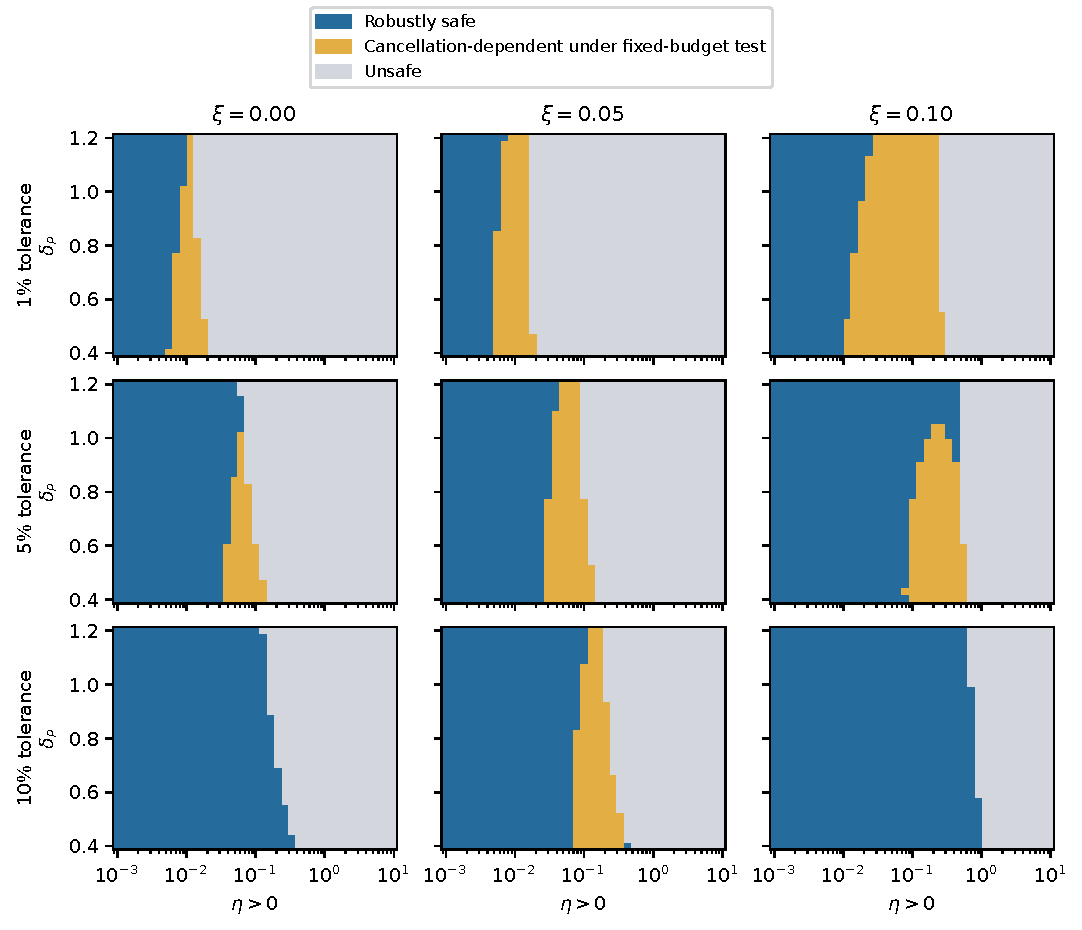
\includegraphics[width=0.96\textwidth]{../figures/main/figure_5_decision_map.pdf}
\caption{Observable-specific omission decisions for $\eta>0$. Rows use 1\%, 5\% and 10\% tolerances; columns use the three Gaussian disorder ranges. Blue is robustly safe, gold is cancellation-dependent under the fixed-budget test, and gray is unsafe. Each row contains the same 3510 positive-coupling points counted in Table~\ref{tab:decisions}; there are no undefined points. Boundaries are sampled, not analytically located. Fixed bands, common texture, $m_P=0$ and $N=256$ are used throughout.}\label{fig:decisions}
\end{figure*}

\subsection{Finite passive curvature}
When a passive mass is allowed, its direct readout must be restored. The correct separation is
\begin{align}
H_{\rm full}-H_0={}&H_P(0,m_P)+[H_A(\eta,m_P)-H_0]\nonumber\\
&+[H_P(\eta,m_P)-H_P(0,m_P)].\label{eq:masssplit}
\end{align}
These are respectively the direct passive baseline, active coupling and passive coupling corrections. For the untilted passive contour,
\begin{equation}
H_P=-\frac{m_Pv_P^2}{2\delta_P^3}(N_+-N_-),\quad
N_s=\sum_{i\in(P,s)}w_i\ell_i.\label{eq:polarization}
\end{equation}
The $N_s$ are driven displacements, not equilibrium densities. Finite-range intrapassive collisions can produce their difference even at $\eta=0$, which a constant-lifetime passive solution would miss.

At $(\delta_P,\xi,m_P)=(0.4,0.1,0.01)$, omission error is already 34.06\% without intersector coupling. At $\eta=0.001$ it is 35.61\%, and the three pieces of Eq.~\eqref{eq:masssplit} are $-2.987834$, $+3.69636\times10^{-5}$ and $-0.211288$. The direct baseline supplies 93.39\% of their absolute budget. The large mass-induced omission is predominantly direct passive readout, rather than active--passive kinetic reshaping. At fixed parameters $H_P/m_P$ approaches finite limits $-299.528$ and $-321.015$ at these two couplings. The mass controls and polarization figure are in the Supplement; no singular zero-mass limit or uniform mass tolerance is inferred.

\subsection{Observable dependence}
Ordinary conductivity makes sector omission a different question for an open-circuit conversion. The partial-channel factors are
\begin{equation}
K_E=-\frac{\chi(\omega)}{\sigma_{yy}(2\omega)},\qquad
K_J=-\frac{\chi(\omega)}{\sigma_{yy}(2\omega)\sigma_{xx}(\omega)^2}.
\end{equation}
The second denominator uses a complex square. Even at $\eta=0$, $m_P=0$, where $H=H_0$ exactly, the passive sector conducts. At $(\delta_P,\xi)=(0.8,0.05)$ the low-frequency ratios are $K_E/K_{E0}=0.26032$ and $K_J/K_{J0}=0.017392$. The derivation and frequency data are supporting results: these factors demonstrate observable dependence within the retained anomalous-velocity channel, not a complete device-voltage prediction.

\section{Discussion}
The reduction separates three questions that a single lifetime or valley count cannot answer. First, does a sector have a direct Hall weight? Second, which physical distributions does its collision coupling excite in the active sector? Third, how accurately must a particular readout be reproduced? A zero answer to the first does not settle the others.

The ablation assigns conditional roles rather than a universal ranking. Active valley distortion carries the retained redistribution coordinate, but only the coupled solution fixes its amplitude. Passive current is indispensable for ordinary conduction and can also alter Hall response. Passive valley polarization closes an additional finite-range feedback path despite having neither direct current nor Hall weight in the massless limit. It is redundant for the driven contact problem and can be unnecessary for a weak-coupling Hall-only tolerance. Four modes provide a common accurate description on the tested domain, not a theorem that every four-valley problem has four relevant modes.

The leakage calculation refines that statement. Contact closure follows from the Bloch-moment structure, while finite range produces a genuinely nonzero invariant residual. Hall accuracy is better than distribution accuracy because projection error is sampled by an observable-specific dual. Compensated drive and leakage forcing, small omitted output sensitivity, and signed modal residues explain the representative errors; uniformly fast leakage does not. Near a tiny net correction, even a small error relative to $|H_0|$ can be a large fraction of that correction. No precision for such a cancellation residual follows from a small total-response error.

These results adapt established sector-reduction and output-error concepts to a specified multivalley anomalous-velocity omission problem. Schur/Kron reduction and adjoint estimation are standard~\cite{DorflerBullo2013,PierceGiles2004}. Valley-polarizing relaxons and scattering-channel subtraction already demonstrate the kinetic content of nonlinear Hall response~\cite{LihmPark2024}. Our contribution is the physically defined ablation, analytic contact closure, quantified finite-range leakage and tolerance-specific distinction between scalar, redistribution and fixed-budget cancellation regimes. Neither the mathematics nor the general importance of valley relaxation is claimed as a priority result.

The physical scope is limited. Side-jump velocities, anomalous distribution terms and skew scattering are excluded and can occur at the same disorder order as the retained channel~\cite{NandySodemann2019,Du2019}. Gaussian disorder removes the third cumulant, not every such contribution; reducing $\Gamma_0$ does not establish a complete Hall response. Kernel and relative-texture controls constrain the present assumptions without demonstrating disorder independence. The bands and disorder ensemble are phenomenological, and the Fermi-contour calculation is at zero temperature. Finite temperature, boundaries and spatial ballistic-to-diffusive transport~\cite{Liu2026} require different calculations. No quantitative SnTe prediction, universal omission threshold or universal enhancement sign follows.

\section{Conclusion}
A Hall-silent conducting sector can matter because its elimination changes both the relaxation and drive of Hall-active distributions. Active reference current and orthogonal valley distortion distinguish scalar rescaling from Hall-sensitive redistribution. Passive current and passive valley polarization transmit their kinetic influence; the latter is essential for the harder finite-range cases but decouples in the massless contact limit.

The specified contact kernel closes analytically on these physical coordinates, with only three driven amplitudes needed. Finite range breaks the factorization of incoming moments and introduces angular outgoing rates. Four modes remain accurate on the tested domain, but their finite leakage is a diagnostic whose observable effect also depends on drive miss, inverse relaxation and Hall overlap. The exact residual identity explains why a small Hall error can coexist with a larger distribution error.

Omission is robustly safe under the fixed-budget test when the absolute component budget cannot exceed the tolerance after favorable signs are removed. Otherwise a safe response can be cancellation-dependent under that test: 571/1410 (40.50\%), 377/1942 (19.41\%) and 136/2201 (6.18\%) of safe positive-coupling points at 1\%, 5\% and 10\%. Finite passive curvature adds a direct population readout that may dominate even before coupling, and conductivity changes the omission decision for open-circuit proxies. The resulting criterion is kinetic, observable specific and tolerance dependent within the anomalous-velocity model. The calculation establishes neither a complete experimental nonlinear Hall conductivity nor a material-independent omission rule.

\section*{Data and code availability}
The accompanying package contains the numerical sources, processed responses, physical-mode ablations, leakage diagnostics and figure inputs. The command \texttt{make reproduce-core} reconstructs the principal response map and targeted analyses; \texttt{make paper} verifies inputs and builds both documents. Complete data definitions and fingerprints are supplied in \texttt{DATA\_MANIFEST.md}.
{\small\setlength{\bibsep}{2pt}\bibliographystyle{unsrtnat}\bibliography{references}}
\end{document}
